\documentclass{article}

\usepackage{graphicx}
\usepackage{hyperref}
\usepackage{titling}
\usepackage{mdframed}
\usepackage{pdflscape}

\setlength{\droptitle}{-25mm}
\title{Product Requirements Document \\ \vspace{1mm} \normalsize For Virtuous Hummingbird}
\author{\href{https://github.com/wintertideheir}{wintertideheir}}
\predate{}
\date{}
\postdate{}

\newcommand{\requirementname}{Undefined}
\newcommand{\requirementlabel}{undefined}
\newcommand{\setreqtype}[2]
    {
        \renewcommand{\requirementname}{#1}
        \renewcommand{\requirementlabel}{#2}
    }
\newenvironment{requirement}[2][]
    {
        \begin{mdframed}
        \label{\requirementlabel-#2}
        \vspace{2.5mm}
        \begin{center}
            {
                \large
                \requirementname\ Requirement #2
            
                #1
            }
        \end{center}
        \vspace{2.5mm}
    }
    {
        \end{mdframed}
    }

\begin{document}

\maketitle
\tableofcontents

\section{Introduction}

Virtuous Hummingbird is a program for the organization and advancement of personal virtue.
By virtue, we mean the virtues of virtue ethics, personal qualities indicating a pattern of repeated behavior.
These qualities are related causally to form a hierarchical tree of virtues. 
The simple nature of virtues and virtue trees makes virtue ethics an unusually intuitive and practical ethical theory.
By presenting a way to create, edit, visualize, and track these virtues, Virtuous Hummingbird facilitates living a virtuous life.

\section{Background}

Virtuous Hummingbird was concieved as an improvement on another concept-mapping system, Cmap, for mapping virtue ethics.

Cmap is a trademark applied to a series of products created by the Florida Institute for Human and Machine Cognition.
Cmap products are intended to empower users to represent knowledge as concept maps.
CmapTools, a Cmap product, is a desktop application that allows users to view and manipulate concept maps.
Because Cmap products could represent any knowledge, CMapTools was adopted as a tool to research virtue ethics.

However, Cmap products are only optimized for general use.
When faced with high volume graphs in virtue ethics, the representations they unnavigatable and unusable.
CmapTools is also limited in it's ability to parse concept maps and generate new insights.
In the long term, CmapTools is not a programs that can be easily extended to perform other functions.

A new kind of concept-mapping software was concieved, optimized for virtue ethics and built with domain-specific utilities.
To avoid information overload, the concept map would be represented as simple nodes defined only be color and position.
The information associated with these nodes would be specific to the virtues of virtue ethics.
Finally, multiple utilities would be built around this base.

\section{Business Requirements}

\begin{landscape}
    \begin{figure}
    \centering
    \def\svgwidth{\columnwidth}
    %% Creator: Inkscape 1.0.2 (e86c870879, 2021-01-15), www.inkscape.org
%% PDF/EPS/PS + LaTeX output extension by Johan Engelen, 2010
%% Accompanies image file 'business.pdf' (pdf, eps, ps)
\begingroup%
  \makeatletter%
  \providecommand\color[2][]{%
    \errmessage{(Inkscape) Color is used for the text in Inkscape, but the package 'color.sty' is not loaded}%
    \renewcommand\color[2][]{}%
  }%
  \providecommand\transparent[1]{%
    \errmessage{(Inkscape) Transparency is used (non-zero) for the text in Inkscape, but the package 'transparent.sty' is not loaded}%
    \renewcommand\transparent[1]{}%
  }%
  \providecommand\rotatebox[2]{#2}%
  \newcommand*\fsize{\dimexpr\f@size pt\relax}%
  \newcommand*\lineheight[1]{\fontsize{\fsize}{#1\fsize}\selectfont}%
  \ifx\svgwidth\undefined%
    \setlength{\unitlength}{1760.25bp}%
    \ifx\svgscale\undefined%
      \relax%
    \else%
      \setlength{\unitlength}{\unitlength * \real{\svgscale}}%
    \fi%
  \else%
    \setlength{\unitlength}{\svgwidth}%
  \fi%
  \global\let\svgwidth\undefined%
  \global\let\svgscale\undefined%
  \makeatother%
  \begin{picture}(1,0.58244568)%
    \lineheight{1}%
    \setlength\tabcolsep{0pt}%
    \put(0,0){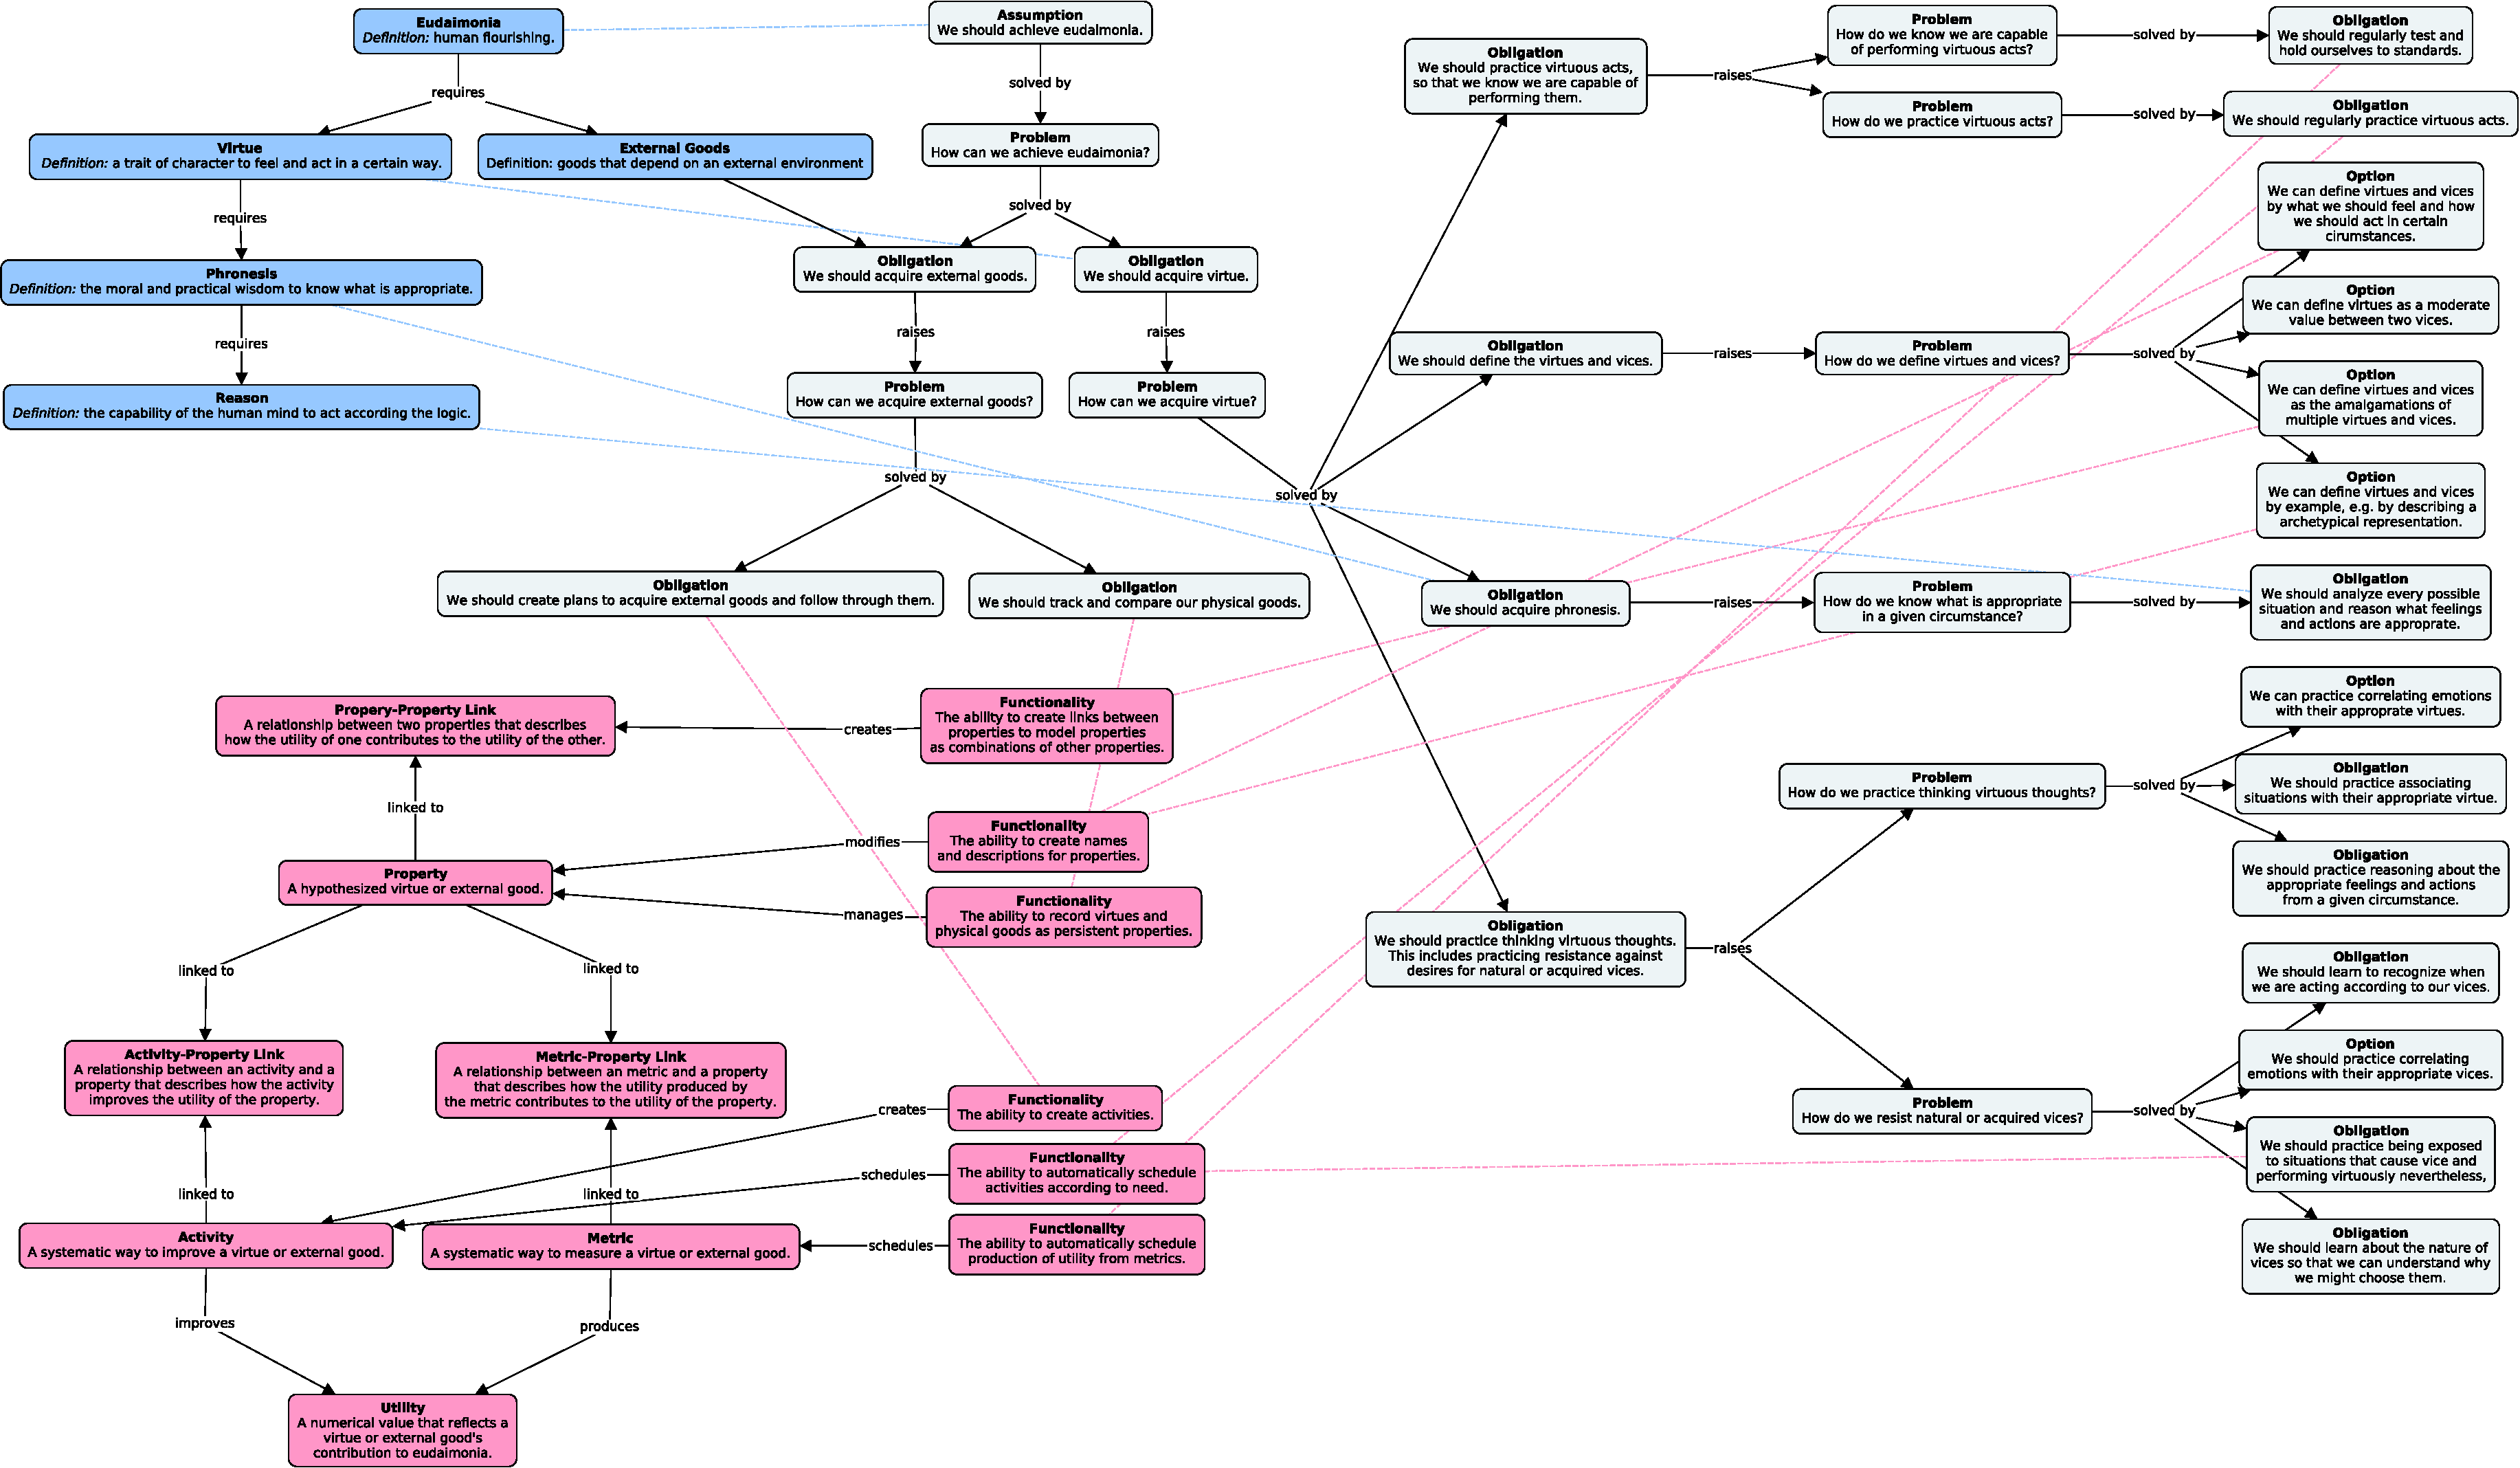
\includegraphics[width=\unitlength,page=1]{business.pdf}}%
  \end{picture}%
\endgroup%

    \label{fig:business}
    \caption{Summary of Business Requirements}
    \end{figure}
\end{landscape}

\section{Market Assessment}

\subsection{Target Demographic}

The target demographic is between 25 and 35 years of age.
This age group has the maturity to recognize the value of an ethical system, and enough time to reap the benefits of a full implementation.

The target demographic is male, because young men appear to take greater risks and have less of a sense of purpose in life.
The downsides of generally greater risk taking can be best mitigated by carefully selecting which risks have the highest return on investment, a task any ethical theory can help with.
Virtue ethics in particular favors long-term develop of the virtues, and therefore uniquely discourages short-term risk-taking.

The target demographic should also be educated, with at least some college, but preferably a bachelor's degree.
Virtue ethics works best when applied to a varied and numerous set of decisions, because their sheer potential complexity requires a deliberately simple approach.
College-educated users manage intellectually challenging classes and/or jobs, which therefore requires managing a varied and numerous set of decisions.

The target demographic is unmarried and without dependents, and preferably single.
As a consequence they will spend less time on relationships that will likely not benefit from ethical theory.

The target demographic values an individualistic approach to life and a Protestant work ethic.
Individualism is the principle that one ought to be independent and self-reliant, which encourages self-directed learning.
The Protestant work ethic is the belief that work, discipline, and frugality are a divine obligation.
A Protestant work ethic requires the hard work needed to make use of virtue ethics.

\subsection{Target Problem}

Our target demographic will likely have problems efficiently managing their time.
In many cases, a combination of a calendar, task-list, and time-tracker can help plan, prioritize, and track their activities.
As the the number and variety of activities increases, however, optimally prioritizing them becomes more difficult.
Virtue ethics can help this problem by offering a long-term, continuous, and simple method of organization.

First, these activities must be integrated into a tree of virtues.
A virtue is a trait with an associated pattern of behavior.
Because nearly all virtues are done for the sake of other virtues, we can represent virtues as a two-dimensional node graph.
The user constructs these virtue trees, assigns initial weights, and then begins recording the consequences of activities.

Virtuous Hummingbird will then learn which virtues the user values the most and present a set of activities that best reflect the virtue tree.
In essence, Virtuous Hummingbird is a form of machine learning applied to task prioritization with an element of deliberation.
By combining hard work and automation, task prioritization is easy.

\subsection{Competing and Comparable Products}

The products that offer the closest functionality to Virtuous Hummingbird are task trackers.
Task trackers expand on the basic task-list with features such as categories, tags, and prioritization.
Their primary advantage is their simplicity of use.
Lists are very simple to create, edit, and view.
Their primary disadvantage is their difficulty in scaling as the number and variety of tasks grows.
Task-trackers attempt to mitigate their scaling problems with organization tools, requiring at least a little planning.
There are several popular task-trackers available as of January 2021:

\begin{description}
    \item[Google Tasks], free.
    A widely used product on account of it being bundled with the standard apps for a Google account.
    It provides the ability to create sub-tasks, set due dates, and send notifications.
    It integrates with other Google apps, namely Gmail and Google Calendar.
    \item[Microsoft To Do], from \$5 per user per month.
    This product appears to offer similar features to Google Tasks.
    \item[Remember The Milk], free or \$40 per year.
    A simple task-list service with a focus on everyday, non-business application.
    Features an advanced auto-complete feature that makes creating tasks convenient.
    It can use e-mail, text, Twitter, and other apps.
    It can connect files from Google Drive and Dropbox to tasks.
    It features a smart search feature and priority system.
    \item[Trello], free to \$17.5 per user per month.
    A professional-focused task tracker.
    Based around dividing tasks into teams.
    These tasks can be detailed with comments, attachments, and due dates, and then viewed with an sophisticated interface.
    Programming and automation is available to streamline that process as well.
    \item[Todoist], free to \$5 per user per month.
    A task-tracker with many interesting features.
    It's core feature are well-detailed tasks.
    It also allows collaboration on tasks, including delegation and comments.
    Gamification is present as well, with a karma system and productivity visualizations.
    \item[Asana], free to per contract pricing.
    A feature-risk task-tracker with many different ways of viewing a task list, including a time-line view, a table view, a multi-list view, etc.
    It also features programming / automation to streamline task creation and management.
\end{description}

Another class of products to consider are time-tracking apps.
Rather than planning an activity in advance, time-tracking apps record an activity as it occurs.
They often have similar features to task-trackers, as well as billing, export, and retrospective editing features.
There are several popular time-tracking apps, as of January 2021:

\begin{description}
    \item[Toggl Track], free or \$9 per user per month.
    An easy-to-use tracking app.
    Activities can be tracked with or without a name, project, or tags, and then edited later.
    It also integrates very well with Google apps and works on many different platforms.
    \item[Harvest], free or \$12 per user per month.
    A team focused time-tracker.
    Teams can connect their logs to an administration log.
    It can also integrate well with task-trackers and other apps.
    \item[Everhour], free or \$5 per user per month.
    A light-weight time-tracker.
    It integrates well with other productivity apps and offers employee integration.
\end{description}

Calendar applications often provide very simple versions of the functionality mentioned above.
Full capability is provided only in conjunction with the above apps.

\section{Product Details}
\subsection{Product Overview}
\subsection{Functional Requirements}
\subsection{Usability Requirements}
\subsection{Technical Requirements}
\subsection{Environmental Requirements}
\section{Supporting Data}
\subsection{Assumptions}
\subsection{Constraints}
\subsection{Dependencies}
\section{Conclusion}

\end{document}
